\textbf{03/04/2025}
\section{Clase 22.}
Problemario p. 35\\

Problema 2.1 Una viga de madera se apoya verticalmente contra un muro. La longitud de la viga es de 30 unidades. Si el extremo superior de la viga se desliza hacia abajo por la pared 6 unidades, ¿cuánto se habrá deslizado el extremo inferior horizontalmente sobre el suelo?

\par
\begin{minipage}[t]{0.66\textwidth}
\textbf{Solución.} 
Por Pitágoras tenemos
$$x=\sqrt{30_{2} - 24_{2}} = \sqrt{324}$$
Luego, calculamos la raiz por el método babilónico
 \begin{gather*}
    a_{1} = 27, a_{2} = 12, a_{3} = \frac{27+12}{2} = 19.5,\\ 
    a_{4} = \frac{324}{19.5} \approx 16.615, \\
    a_{5} = \frac{19.5+16.615}{2} = 18.0575\\
    a_{6} = \frac{324}{18.0575} \approx 17.9426,\\
    a_{7} = \frac{17.9426+18.0575}{2} = 18.00005\\
    a_{8} = \frac{324}{18.00005} = 17.99995,\\
    a_{9} = \frac{18.00005+17.99995}{2} = 18, \\
    a_{10} = \frac{324}{18} = 18
 \end{gather*}
Así, la viga se deslizó horizontalmente 18 unidades.
\end{minipage}
\begin{minipage}[t]{0.3\textwidth}
    \centering
    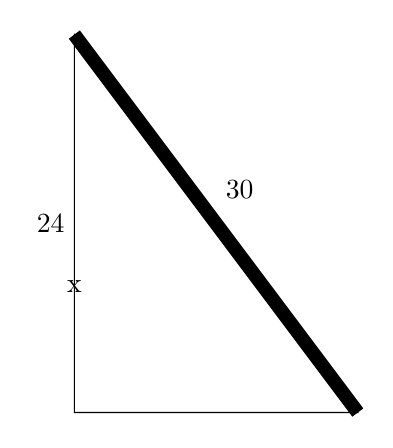
\begin{tikzpicture}[baseline=(current bounding box.north), scale = 2]
    \coordinate (A) at (0,0);
    \coordinate (B) at (1.8,0);
    \coordinate (C) at (0,2.4);

    \draw (A) -- (B) -- (C) --cycle;
    \draw[line width=5pt] (B) -- (C);
    \node[left] at (0,1.2) {24};
    \node[above right] at (0.9,1.3) {30};
    \node[below] at (0,0.9) {x};
    
\end{tikzpicture}
\end{minipage}
\par

\subsection{Proporción aurea}

\subsection{Pi}